\documentclass[aspectratio=169,11pt]{beamer}
\usepackage{teaching_slides}


\begin{document}

\title[Econometrics I]{ Econometrics I}
\subtitle{Lecture 11: Count Data}
\author{Chris Conlon \\NYU Stern}
\date{\today}
\maketitle


\begin{frame}
\frametitle{Count Data}
\begin{itemize}
\item Dependent variable measures a count $y = 0,1,2,\dots$

\medskip
\item Examples: number of units purchased, number of doctor visits, number of children (fertility).


\end{itemize}
\end{frame}



\begin{frame}
\frametitle{Poisson distribution}
\begin{itemize}
\item {\bf Poisson process}: events happen independently over time at rate $\lambda$
	per unit time. The {\bf Poisson distribution} gives the distribution over the number of events
	that happen.

	\smallskip
	\item Probability mass:\[
		Pr\left(Y=y \mid \lambda\right) = \frac{e^{-\lambda}\lambda^{y}}{y!}
	\]

	The Poisson distribution just has one parameter:\begin{align*}
	\E\left[y\right] & = \lambda \\
	\Var\left[y\right] &= \lambda
	\end{align*}

	\item The Poisson distribution features {\bf equidispersion}, mean$ = $variance. \\
	\item It's more common to see {\bf overdispersion} in count data (variance$>$mean) (which sometimes leads to \textit{negative binomial} models).
\end{itemize}
\end{frame}



\begin{frame}
\frametitle{Poisson distribution}
\begin{center}
 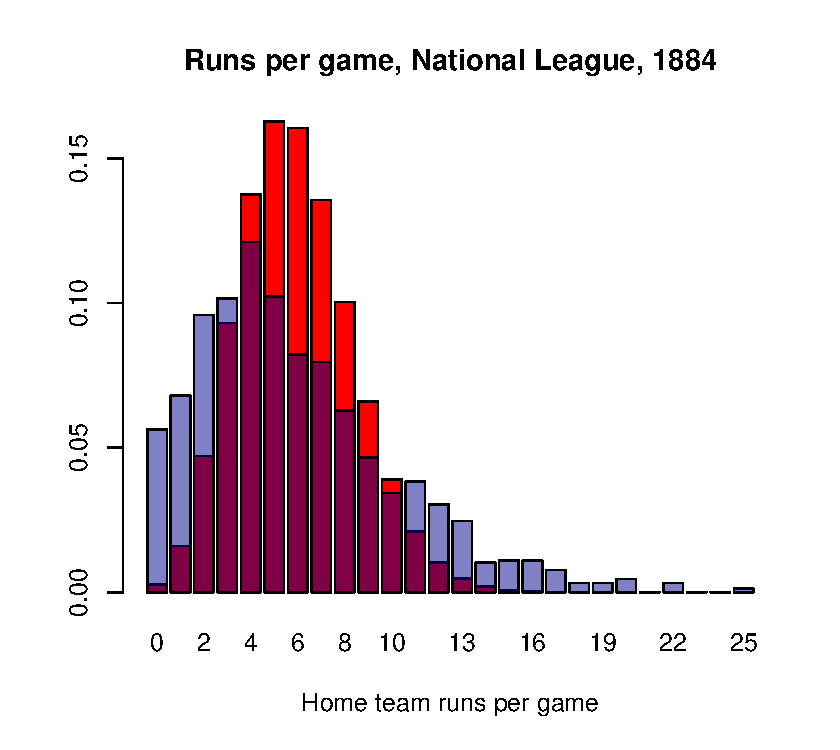
\includegraphics[height=.7\textheight]{./resources/home_team_runs}
\end{center}
{\small
Plotted Poisson distribution (red) is for $\lambda$ equal to the average runs per game. \\
Empirical probability mass function is in blue. 
}
\end{frame}




\begin{frame}
\frametitle{Poisson regression (MLE)} 
\begin{itemize}
\item  Let the Poisson rate vary with observable characteristics ${\bf x}$:\[
	\lambda \left({\bf x}\right) = \E\left[y \mid {\bf x}\right] = \exp\left({\bf x}'\symbf{\beta}\right).
	\]
	Note that this ensures that $\lambda\left({\bf x}\right) > 0$.

	\medskip
	\item Log likelihood follows from Poisson pdf:\begin{align*}
	\ell\left(y,\boldsymbol{x} \right) & =  \frac{e^{-\lambda}\lambda^{y}}{y!} \\
	\ln \ell\left(y,{\bf x}\right) &= -\exp\left({\bf x}'\symbf{\beta}\right) + y{\bf x}'\symbf{\beta} - \ln y! \\
	\ln L\left(\symbf{\beta} \mid {\bf y},{\bf X}\right) &=  \sum_{i=1}^{n}\left\{-\exp\left({\bf x}_{i}'\symbf{\beta} \right)+ y_i{\bf x}_{i}' \symbf{\beta} +\ln y_{i}!\right\}
	\end{align*}
\end{itemize}
\end{frame}


\begin{frame}
\frametitle{Poisson regression (MLE)} 
\begin{itemize}
	\item Log likelihood:\[
	\ln L\left(\symbf{\beta} \mid {\bf y},{\bf X}\right) =  \sum_{i=1}^{n}\left\{-\exp\left({\bf x}_{i}'\symbf{\beta} \right)+ y_i{\bf x}_{i}' \symbf{\beta} +\ln y_{i}!\right\}
	\]

	\item First-order condition for maximum:\begin{align*}
	  \sum_{i=1}^{n}\left\{-\exp\left({\bf x}_{i}'\symbf{\beta} \right) {\bf x}_{i} + y_i{\bf x}_{i} \right\} & =0\\
  \sum_{i=1}^{n}\left\{\left(y_i -\exp\left({\bf x}_{i}'\symbf{\beta} \right) \right) {\bf x}_{i} \right\} & =0
	\end{align*}

	\item Log likelihood function is globally concave, so computer will generally converge to solution quickly.
\end{itemize}
\end{frame}




\begin{frame}
\frametitle{Poisson model: marginal effects} 
\begin{itemize}
\item Marginal effects are given by\[
	\frac{\partial \E\left[y \mid {\bf x}\right]}{\partial x_j} = \exp\left( {\bf x}'\symbf{\beta}\right) \beta_j =
	\E\left[y \mid {\bf x}\right] \beta_j 
\]

	\item Alternatively,\[
	\frac{1}{\E\left[y \mid {\bf x}\right] }\frac{\partial \E\left[y \mid {\bf x}\right]}{\partial x_j}  = \beta_j,
\]
which makes it clear that coefficients can be interpreted as proportional change in mean for one unit change in covariate $x_j$. 


\end{itemize}
\end{frame}



\begin{frame}
\frametitle{Poisson regression consistency} 
\begin{itemize}
	\item First-order condition for maximum:\[
  \sum_{i=1}^{n}\left\{\left(y_i -\exp\left({\bf x}_{i}'\symbf{\beta} \right) \right) {\bf x}_{i} \right\} =0
	\]

	\smallskip
	\item Note this moment condition is satisfied if $\E\left[y_i \mid {\bf x}_i\right] = \exp\left({\bf x}_{i}'\symbf{\beta}\right)$.

	\smallskip
	\item MLE estimation consistent even if $\Var\left[y_i \mid {\bf x}_i\right] \ne \exp\left({\bf x}_{i}'\symbf{\beta}\right)$. 

	\smallskip
	\item $\Rightarrow$ we might want to estimate Poisson MLE even if we don't believe in equidispersion.
\end{itemize}
\end{frame}



\begin{frame}
\frametitle{Poisson regression standard errors} 
\begin{itemize}
	\item If we don't want to impose equidispersion, then we shouldn't rely on MLE standard errors;
	we should instead look at this as GMM estimation, and compute
	standard errors using standard sandwich formula (more on this next semester).

	\smallskip
	\item With equidispersion (full Poisson model), see MLE slides for standard errors formulas.

	\smallskip
	\item There can be a big difference between the two!
\end{itemize}
\end{frame}


\begin{frame}
\frametitle{Poisson Generalized linear model} 
\begin{itemize}
	\item Instead of imposing $\Var\left[y \mid {\bf x}\right] = \E\left[y | {\bf x}\right]$, we can let \[
		\Var\left[y \mid {\bf x}\right] =  \gamma \E\left[y \mid {\bf x}\right] = \gamma\exp\left( {\bf x}_{i}'\symbf{\beta} \right),
	\]
	and estimate\[
	\hat{\gamma} = \frac{1}{n-k} \sum_i \frac{\left(y_i - \exp\left( {\bf x}_{i}'\symbf{\beta} \right)\right)^2}{\exp\left( {\bf x}_{i}'\symbf{\beta} \right)}.
	\]
	Note that this is just a standard estimator of the variance, divided by our formula for the mean.

	\item This makes sense for \emph{estimation}, and $\gamma$ can be used in sandwich estimator for consistent standard errors.
			But what about for \emph{simulation} -- what is the distribution of the data generating process with $\gamma \ne 1$?
			

\end{itemize}
\end{frame}








\begin{frame}
\frametitle{Negative binomial distribution}
\begin{itemize}
\item  Let
\begin{align*}
	y & \sim Poisson\left[\lambda \nu \right] \\
	\nu & \sim Gamma\left[\mu = 1, \sigma^2 =\alpha \right].
\end{align*}
	Then we say that $y$ has a negative binomial distribution with mean $\lambda$ and variance $\lambda +\alpha \lambda^2$.

	\item The negative binomial distribution is typically described as the number of failures observed before
			we see $r$ successes when doing independent Bernoulli trials with success rate $p$. The above has the same distribution
			as $r=\frac{1}{\alpha}$ and $p = \frac{\lambda \alpha}{1+\lambda \alpha}$. 

	\item Note that, with either of the above descriptions, it's easy to describe and simulate the full distribution or data generating process (you can
look up the distribution functions on Wikipedia).



\end{itemize}
\end{frame}


\begin{frame}
\frametitle{Negative binomial distribution: estimation}
\begin{itemize}
	\item When we're worried about overdispersion, it makes sense to assume a negative binomial distribution instead of a simple Poisson.

	\smallskip
	\item We could use MLE for the negative binomial distribution. This is the most efficient thing if the specification is correct (MLE is always
		asymptotically efficient for correctly specified models).

	\smallskip
	\item However, we could still do Poisson regression (noting that the negative negative binomial extension does not change the mean, and Poisson
	regression is consistent as long as mean is correctly specified). In this, can estimate model of (conditional) mean using Poisson regression.
	
	\smallskip
	\item If you're only interested in how the mean of $y$ depends on $x$, you're done after estimating a Poisson regression. If you want to do simulations or 
		compute standard
		errors on the variance parameter (robust to overdispersion), you should estimate the negative binomial model using a GMM or MLE estimator. 

\end{itemize}
\end{frame}





\begin{frame}
\frametitle{Further comments}
\begin{itemize}
	\item Poisson is nested within negative binomial with $\alpha=0$. Thus, likelihood ratio test applies and effectively serves as a test
		for overdispersion.

	\item As Lancaster (1997) points out, Poisson model with fixed effects has incidental parameters, but they are not problematic.
	\begin{itemize}
		\item Recall in binary choice logit model, we can handle fixed effects by constructing conditional likelihood function. For Poisson models,
		we can just use the regular likelihood function with fixed effects, and those fixed effects don't create a problem for our standard errors.
		The Poisson model and linear regression model have this in common. 
	\end{itemize}
	
	\item Poisson regression can be used for things that don't have the Poisson distribution's equidispersion, but you
				shouldn't use the MLE estimator's standard errors in that case. 
\end{itemize}
\end{frame}


\begin{frame}
\begin{center}
Text Analysis
\end{center}
\end{frame}


\begin{frame}
\frametitle{Overview}
\begin{itemize}
\item \href{https://web.stanford.edu/~gentzkow/research/text-as-data.pdf}{Gentzkow, Kelly, and Taddy (2019)} provides
	a good overview from a social science perspective. 

	\item Text analysis generally built on either {\bf multinomial choice models} (there is a probability distribution over what each word is) or 
		{\bf count data models} (there is a probability distribution over counts of words or phrases). 

	\item It's common to model different distributions for different topics. For example, in the latent Dirilichet allocation,
 	\begin{itemize}
		\item Documents are drawn from topics. A probability distribution over topics is estimated. We don't pre-specify what the topics are 
			({\bf unsupervised learning}), though we might pre-specify the number of topics.

		\item Each topic is associated with a probability distribution over words (which we estimate). 

		\item Post-estimation, the topics can typically be interpreted based on which words have relatively high frequencies. Application: grouping papers or
			patent applications by field. 

	\end{itemize}
\end{itemize}
\end{frame}




\begin{frame}
\begin{center}
Gentzkow, Shapiro, and Taddy (2019) 
\end{center}
\end{frame}



\begin{frame}
\frametitle{Overview}
\begin{itemize}
\item Measuring divergence in speech patterns of US political parties. ``Speaking
different languages.'' 

\smallskip
\item Documents increasing partisanship since 1994 (Newt Gingrich).
		 A rare example of great descriptive econometrics. 

\small
\item Challenges:
\begin{itemize}
	\item There are lots of words, many of them used very rarely.
	\item Standard multinomial logit model computationally intractible.
\end{itemize}
\end{itemize}
\end{frame}



\begin{frame}
\frametitle{Setup}
\begin{itemize}
\item ${\bf x}_{i,t}$ is a vector of speaker $i$'s characteristics in session $t$.
\begin{itemize}
	\item state, chamber, gender
\end{itemize}

\smallskip
\item  ${\bf q}_t^P\left({\bf x}_{i,t}\right)$ is a  $J$-dimensional (very large) vector of probabilities
		of using phrases. $P\in \left\{R,D\right\}$ denotes party.

\smallskip
\item We're interested in whether ${\bf q}_t^D$ differs from ${\bf q}_t^R$, and whether
		the difference between the two increases over time.
\end{itemize}
\end{frame}

\begin{frame}
\frametitle{Partisanship}
\begin{itemize}
\item Define\[
	\rho_{jt}\left({\bf x}\right) =\frac{q_{jt}^R\left({\bf x}\right)}{q_{jt}^R\left({\bf x}\right) + q_{jt}^D\left({\bf x}\right)}
\]
\[
	\boldsymbol{\pi}_{t} \left({\bf x}\right) =\frac{1}{2}{\bf q}_t^R\left({\bf x}\right) \cdot \boldsymbol{\rho}_{t} \left({\bf x}\right)
		+\frac{1}{2} {\bf q}_t^D\left({\bf x}\right) \cdot \left(1- \boldsymbol{\rho}_{t} \left({\bf x}\right)\right)
\]

\item $\rho_{jt}\left({\bf x}\right)$ is poserior probability that phrase $j$ at time $t$ comes from Republican. 

\item $\pi_{t} \left({\bf x}\right)$ aggregates these probabilities a natural measure of the partisanship. It's the probability
			you can guess the speaker's party correctly if they have characteristics $\boldsymbol{x}$. $\bar{\pi}_t$
			then averages over $\boldsymbol{x}$.
			
\end{itemize}
\end{frame}


\begin{frame}
\frametitle{Small-sample bias}
\begin{center}
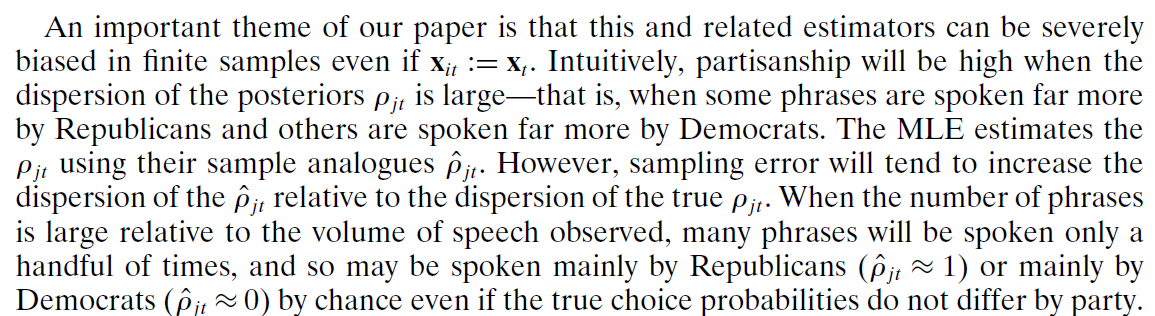
\includegraphics[width=.8\textwidth]{./resources/GST_bias}
\end{center}
\end{frame}



\begin{frame}
\frametitle{Avoiding bias}
\begin{enumerate}
\item {\bf Leave-out estimator}: Estimate $ {\bf q}_t$ and $\boldsymbol{\rho}_t$ using different samples.

\item {\bf Penalized estimator}: parameterized choice model. Like Lasso, incorporate penalty for each non-zero parameter.
\begin{itemize}
\item Instead of multinomial logit estimator of frequencies, use Poisson model of counts. Note that Poisson
		mean $\exp\left({\bf x}' \symbf{\beta}\right)$ is also the numerator of a logit model. Apparently
		avoiding the need to compute the denominator is a big deal computationally. 
\end{itemize}		
			
\end{enumerate}
\end{frame}


% note: during 20th century, verbosity increased

\begin{frame}
\begin{center}
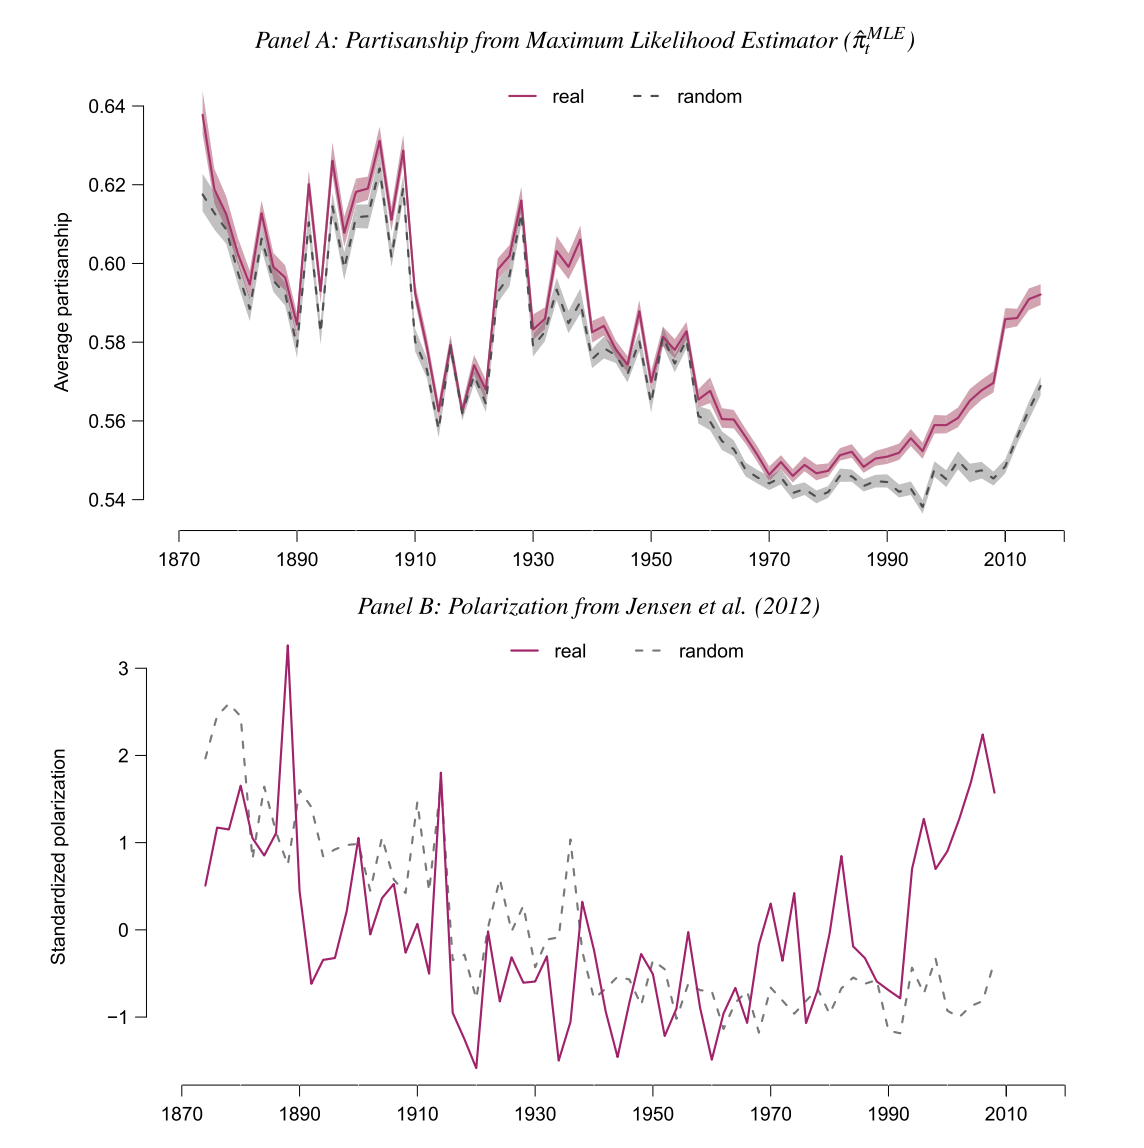
\includegraphics[height=.9\textheight]{./resources/GST_results1}
\end{center}
\end{frame}

\begin{frame}
\begin{center}
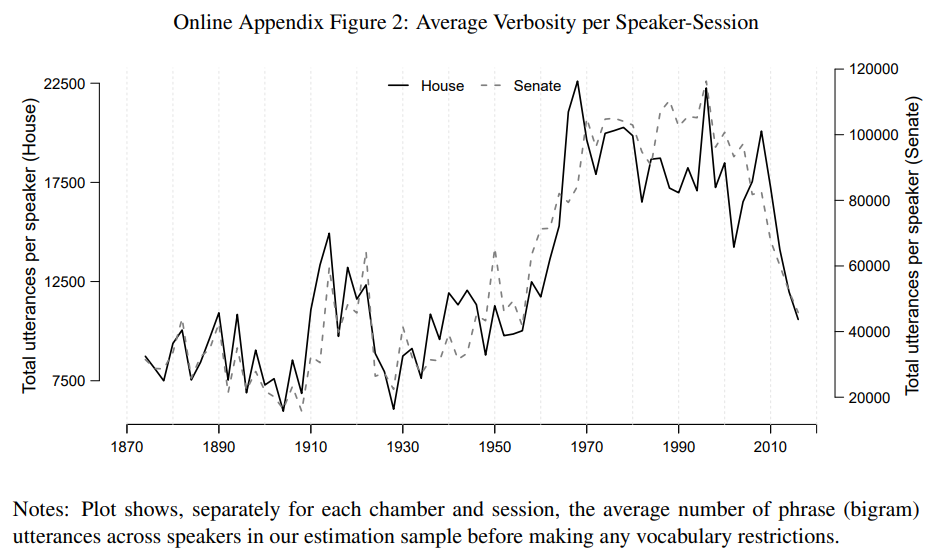
\includegraphics[height=.9\textheight]{./resources/GST_verbosity}
\end{center}
\end{frame}

\begin{frame}
\begin{center}
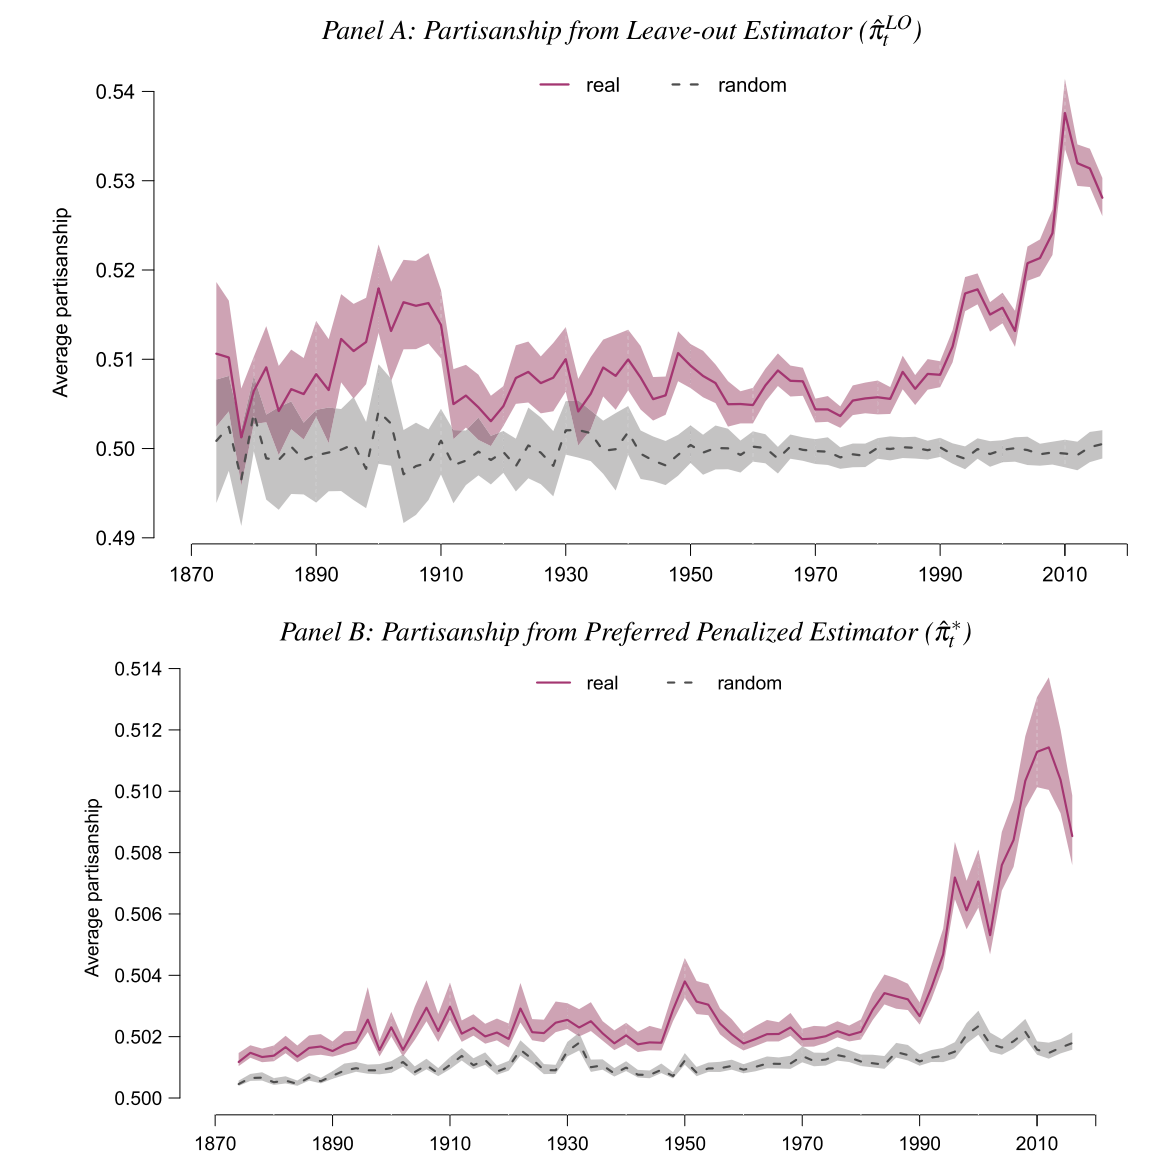
\includegraphics[height=.9\textheight]{./resources/GST_results2}
\end{center}
\end{frame}

\end{document}
